
%(BEGIN_QUESTION)
% Copyright 2010, Tony R. Kuphaldt, released under the Creative Commons Attribution License (v 1.0)
% This means you may do almost anything with this work of mine, so long as you give me proper credit

Suppose a technician connects a voltmeter and an ammeter to the three-phase conductors of an running electric motor as shown in this simplified illustration (all control wiring has been omitted for simplicity):

$$\includegraphics[width=15.5cm]{i02258x01.eps}$$

Calculate the mechanical horsepower output of this motor, assuming 91\% efficiency and perfect power factor.

\vfil 

\underbar{file i02258}
\eject
%(END_QUESTION)





%(BEGIN_ANSWER)

This is a graded question -- no answers or hints given!

%(END_ANSWER)





%(BEGIN_NOTES)

With a perfect power factor, apparent power and true power will be the same (Volt-Amps = Watts).  Thus, we may calculate true power ($P$) using scalar quantities of 463.2 volts and 18.5 amps:

$$P_{total} = \sqrt{3} (I_{line}) (V_{line})$$

$$P_{total} = \sqrt{3} (18.5) (463.2)$$

$$P_{total} = 14,842.3 \hbox{ watts}$$

Given the equivalence of 746 watts to 1 horsepower, this yields a figure of 19.896 HP of electrical power.  However, since the motor's stated efficiency rating of 91\% means only 91\% of this electrical power actually gets converted into mechanical shaft power, the mechanical output of this electric motor will be less than the amount of electrical power we just calculated:

\vskip 10pt

(19.896 HP)(0.91) = 18.105 horsepower of mechanical power at the shaft

\vskip 10pt

A common error made by students is to apply the efficiency figure incorrectly, dividing by 0.91 instead of multiplying by 0.91.  A fundamental principle to bear in mind here is the {\it Law of Energy Conservation}, which states that energy cannot be created or destroyed, but may only be converted from one form to another.  In the case of an electric motor, the incoming electrical energy will be mostly converted into outgoing mechanical (shaft) energy, with a small fraction converted into heat.  The sum total of mechanical power and heat losses must equal the total electrical energy sent to the motor, in accordance with the {\it Conservation of Energy}.  This logically means the mechanical power output by the motor must be {\it less} than the electrical power input to the motor.  

You should always qualitatively check your answer(s) against this principle, to ensure you are properly applying the efficiency figure.  The power output by any energy-conversion machine can never be greater than the amount of power it receives!

%INDEX% Electronics review: 3-phase electrical power 

%(END_NOTES)

